
\documentclass[letterpaper,hide notes,xcolor={table,svgnames},pdftex,10pt]{beamer}
\def\showexamples{t}


%\usepackage[svgnames]{xcolor}

%% Demo talk
%\documentclass[letterpaper,notes=show]{beamer}

\usecolortheme{crane}
\setbeamertemplate{navigation symbols}{}

\usetheme{MyPittsburgh}
%\usetheme{Frankfurt}

%\usepackage{tipa}

\usepackage{hyperref}
\usepackage{graphicx,xspace}
\usepackage[normalem]{ulem}
\usepackage{multicol}
\usepackage{amsmath,amssymb,amsthm,graphicx,xspace}
\newcommand\SF[1]{$\bigstar$\footnote{SF: #1}}

\usepackage[default]{sourcesanspro}
\usepackage[T1]{fontenc}
\usepackage[scaled]{beramono}
\usepackage{tikzpagenodes}

\newcounter{tmpnumSlide}
\newcounter{tmpnumNote}


% old question code
%\newcommand\question[1]{{$\bigstar$ \small \onlySlide{2}{#1}}}
% \newcommand\nquestion[1]{\ifdefined \presentationonly \textcircled{?} \fi \note{\par{\Large \textbf{?}} #1}}
% \newcommand\nanswer[1]{\note{\par{\Large \textbf{A}} #1}}


 \newcommand\mnote[1]{%
   \addtocounter{tmpnumSlide}{1}
   \ifdefined\showcues {~\tiny\fbox{\arabic{tmpnumSlide}}}\fi
   \note{\setlength{\parskip}{1ex}\addtocounter{tmpnumNote}{1}\textbf{\Large \arabic{tmpnumNote}:} {#1\par}}}

\newcommand\mmnote[1]{\note{\setlength{\parskip}{1ex}#1\par}}

%\newcommand\mnote[2][]{\ifdefined\handoutwithnotes {~\tiny\fbox{#1}}\fi
% \note{\setlength{\parskip}{1ex}\textbf{\Large #1:} #2\par}}

%\newcommand\mnote[2][]{{\tiny\fbox{#1}} \note{\setlength{\parskip}{1ex}\textbf{\Large #1:} #2\par}}

\newcommand\mquestion[2]{{~\color{red}\fbox{?}}\note{\setlength{\parskip}{1ex}\par{\Large \textbf{?}} #1} \note{\setlength{\parskip}{1ex}\par{\Large \textbf{A}} #2\par}\ifdefined \presentationonly \pause \fi}

\newcommand\blackboard[1]{%
\ifdefined   \showblackboard
  {#1}
  \else {\begin{center} \fbox{\colorbox{blue!30}{%
         \begin{minipage}{.95\linewidth}%
           \hspace{\stretch{1}} Some space intentionally left blank; done at the blackboard.%
         \end{minipage}}}\end{center}}%
         \fi%
}



%\newcommand\q{\tikz \node[thick,color=black,shape=circle]{?};}
%\newcommand\q{\ifdefined \presentationonly \textcircled{?} \fi}

\usepackage{listings}
\lstset{basicstyle=\footnotesize\ttfamily,
	breaklines=true,
	aboveskip=15pt,
  	belowskip=15pt,
	frame=lines,
	numbers=left, basicstyle=\scriptsize, numberstyle=\tiny, stepnumber=0, numbersep=2pt
}

\usepackage{siunitx}
\newcommand\sius[1]{\num[group-separator = {,}]{#1}\si{\micro\second}}
\newcommand\sims[1]{\num[group-separator = {,}]{#1}\si{\milli\second}}
\newcommand\sins[1]{\num[group-separator = {,}]{#1}\si{\nano\second}}
\sisetup{group-separator = {,}, group-digits = true}

%% -------------------- tikz --------------------
\usepackage{tikz}
\usetikzlibrary{positioning}
\usetikzlibrary{arrows,backgrounds,automata,decorations.shapes,decorations.pathmorphing,decorations.markings,decorations.text,decorations.pathreplacing}

\tikzstyle{place}=[circle,draw=blue!50,fill=blue!20,thick, inner sep=0pt,minimum size=6mm]
\tikzstyle{transition}=[rectangle,draw=black!50,fill=black!20,thick, inner sep=0pt,minimum size=4mm]

\tikzstyle{block}=[rectangle,draw=black, thick, inner sep=5pt]
\tikzstyle{bullet}=[circle,draw=black, fill=black, thin, inner sep=2pt]

\tikzstyle{pre}=[<-,shorten <=1pt,>=stealth',semithick]
\tikzstyle{post}=[->,shorten >=1pt,>=stealth',semithick]
\tikzstyle{bi}=[<->,shorten >=1pt,shorten <=1pt, >=stealth',semithick]

\tikzstyle{mut}=[-,>=stealth',semithick]

\tikzstyle{treereset}=[dashed,->, shorten >=1pt,>=stealth',thin]

\usepackage{ifmtarg}
\usepackage{xifthen}
\makeatletter
% new counter to now which frame it is within the sequence
\newcounter{multiframecounter}
% initialize buffer for previously used frame title
\gdef\lastframetitle{\textit{undefined}}
% new environment for a multi-frame
\newenvironment{multiframe}[1][]{%
\ifthenelse{\isempty{#1}}{%
% if no frame title was set via optional parameter,
% only increase sequence counter by 1
\addtocounter{multiframecounter}{1}%
}{%
% new frame title has been provided, thus
% reset sequence counter to 1 and buffer frame title for later use
\setcounter{multiframecounter}{1}%
\gdef\lastframetitle{#1}%
}%
% start conventional frame environment and
% automatically set frame title followed by sequence counter
\begin{frame}%
\frametitle{\lastframetitle~{\normalfont(\arabic{multiframecounter})}}%
}{%
\end{frame}%
}
\makeatother

\makeatletter
\newdimen\tu@tmpa%
\newdimen\ydiffl%
\newdimen\xdiffl%
\newcommand\ydiff[2]{%
    \coordinate (tmpnamea) at (#1);%
    \coordinate (tmpnameb) at (#2);%
    \pgfextracty{\tu@tmpa}{\pgfpointanchor{tmpnamea}{center}}%
    \pgfextracty{\ydiffl}{\pgfpointanchor{tmpnameb}{center}}%
    \advance\ydiffl by -\tu@tmpa%
}
\newcommand\xdiff[2]{%
    \coordinate (tmpnamea) at (#1);%
    \coordinate (tmpnameb) at (#2);%
    \pgfextractx{\tu@tmpa}{\pgfpointanchor{tmpnamea}{center}}%
    \pgfextractx{\xdiffl}{\pgfpointanchor{tmpnameb}{center}}%
    \advance\xdiffl by -\tu@tmpa%
}
\makeatother
\newcommand{\copyrightbox}[3][r]{%
\begin{tikzpicture}%
\node[inner sep=0pt,minimum size=2em](ciimage){#2};
\usefont{OT1}{phv}{n}{n}\fontsize{4}{4}\selectfont
\ydiff{ciimage.south}{ciimage.north}
\xdiff{ciimage.west}{ciimage.east}
\ifthenelse{\equal{#1}{r}}{%
\node[inner sep=0pt,right=1ex of ciimage.south east,anchor=north west,rotate=90]%
{\raggedleft\color{black!50}\parbox{\the\ydiffl}{\raggedright{}#3}};%
}{%
\ifthenelse{\equal{#1}{l}}{%
\node[inner sep=0pt,right=1ex of ciimage.south west,anchor=south west,rotate=90]%
{\raggedleft\color{black!50}\parbox{\the\ydiffl}{\raggedright{}#3}};%
}{%
\node[inner sep=0pt,below=1ex of ciimage.south west,anchor=north west]%
{\raggedleft\color{black!50}\parbox{\the\xdiffl}{\raggedright{}#3}};%
}
}
\end{tikzpicture}
}


%% --------------------

%\usepackage[excludeor]{everyhook}
%\PushPreHook{par}{\setbox0=\lastbox\llap{MUH}}\box0}

%\vspace*{\stretch{1}

%\setbox0=\lastbox \llap{\textbullet\enskip}\box0}

\setlength{\parskip}{\fill}

\newcommand\noskips{\setlength{\parskip}{1ex}}
\newcommand\doskips{\setlength{\parskip}{\fill}}

\newcommand\xx{\par\vspace*{\stretch{1}}\par}
\newcommand\xxs{\par\vspace*{2ex}\par}
\newcommand\tuple[1]{\langle #1 \rangle}
\newcommand\code[1]{{\sf \footnotesize #1}}
\newcommand\ex[1]{\uline{Example:} \ifdefined \presentationonly \pause \fi
  \ifdefined\showexamples#1\xspace\else{\uline{\hspace*{2cm}}}\fi}

\newcommand\ceil[1]{\lceil #1 \rceil}


\AtBeginSection[]
{
   \begin{frame}
       \frametitle{Outline}
       \tableofcontents[currentsection]
   \end{frame}
}



\pgfdeclarelayer{edgelayer}
\pgfdeclarelayer{nodelayer}
\pgfsetlayers{edgelayer,nodelayer,main}

\tikzstyle{none}=[inner sep=0pt]
\tikzstyle{rn}=[circle,fill=Red,draw=Black,line width=0.8 pt]
\tikzstyle{gn}=[circle,fill=Lime,draw=Black,line width=0.8 pt]
\tikzstyle{yn}=[circle,fill=Yellow,draw=Black,line width=0.8 pt]
\tikzstyle{empty}=[circle,fill=White,draw=Black]
\tikzstyle{bw} = [rectangle, draw, fill=blue!20, 
    text width=4em, text centered, rounded corners, minimum height=2em]
    
    \newcommand{\CcNote}[1]{% longname
	This work is licensed under the \textit{Creative Commons #1 3.0 License}.%
}
\newcommand{\CcImageBy}[1]{%
	\includegraphics[scale=#1]{creative_commons/cc_by_30.pdf}%
}
\newcommand{\CcImageSa}[1]{%
	\includegraphics[scale=#1]{creative_commons/cc_sa_30.pdf}%
}
\newcommand{\CcImageNc}[1]{%
	\includegraphics[scale=#1]{creative_commons/cc_nc_30.pdf}%
}
\newcommand{\CcGroupBySa}[2]{% zoom, gap
	\CcImageBy{#1}\hspace*{#2}\CcImageNc{#1}\hspace*{#2}\CcImageSa{#1}%
}
\newcommand{\CcLongnameByNcSa}{Attribution-NonCommercial-ShareAlike}

\newenvironment{changemargin}[1]{% 
  \begin{list}{}{% 
    \setlength{\topsep}{0pt}% 
    \setlength{\leftmargin}{#1}% 
    \setlength{\rightmargin}{1em}
    \setlength{\listparindent}{\parindent}% 
    \setlength{\itemindent}{\parindent}% 
    \setlength{\parsep}{\parskip}% 
  }% 
  \item[]}{\end{list}} 




% Custom packages
\usepackage{xcolor}
\definecolor{solarizedBase03}{HTML}{FFFFFF}
\definecolor{solarizedBase02}{HTML}{000000}
\definecolor{solarizedBase00}{HTML}{657B83}
\definecolor{solarizedBase0}{HTML}{000000}
\definecolor{solarizedBase1}{HTML}{93A1A1}
\definecolor{solarizedBase3}{HTML}{FDF6E3}


\usepackage[listings]{tcolorbox}
\newtcbinputlisting{\codelisting}[2][]{
    listing file={#2},
    colback=solarizedBase03,
    colframe=solarizedBase02,
    colupper=solarizedBase0,
    fonttitle=\bfseries\color{solarizedBase1},
    listing options={basicstyle=\ttfamily\footnotesize},
    listing only,
    #1
}
\newtheorem{defn}{Definition}

\title{Lecture 23 --- Password Cracking, Reduced-Resource Computation }

\author{Patrick Lam \& Jeff Zarnett \\ \small \texttt{patrick.lam@uwaterloo.ca}, \texttt{jzarnett@uwaterloo.ca}}
\institute{Department of Electrical and Computer Engineering \\
  University of Waterloo}
\date{\today}


\begin{document}

\begin{frame}
  \titlepage

 \end{frame}


%%%%%%%%%%%%%%%%%%%%%%%%%%%%%%%%%%%%%%%%%%%%%%%%%%%%%%%%%%%%%%%%%%%%%%%%%%%%%%%%
\begin{frame}
  \frametitle{Reference: scrypt}

  
    scrypt is the algorithm behind DogeCoin. \\[1em] The reference:\\[1em]
    
    Colin Percival, ``Stronger Key Derivation via Sequential Memory-Hard Functions''. \\
    Presented at BSDCan'09, May~2009.\\[1em]

    \url{http://www.tarsnap.com/scrypt.html}
  
\end{frame}
%%%%%%%%%%%%%%%%%%%%%%%%%%%%%%%%%%%%%%%%%%%%%%%%%%%%%%%%%%%%%%%%%%%%%%%%%%%%%%%%

%%%%%%%%%%%%%%%%%%%%%%%%%%%%%%%%%%%%%%%%%%%%%%%%%%%%%%%%%%%%%%%%%%%%%%%%%%%%%%%%
\begin{frame}
  \frametitle{Acceptable Practices for Password Storage}
  
    \begin{itemize}
    \item {\Huge \alert{{\bf not} plaintext!}}
    \item \Large hashed and salted
    \end{itemize}
       

\end{frame}
%%%%%%%%%%%%%%%%%%%%%%%%%%%%%%%%%%%%%%%%%%%%%%%%%%%%%%%%%%%%%%%%%%%%%%%%%%%%%%%%

%%%%%%%%%%%%%%%%%%%%%%%%%%%%%%%%%%%%%%%%%%%%%%%%%%%%%%%%%%%%%%%%%%%%%%%%%%%%%%%%
\begin{frame}
  \frametitle{Cryptographic hashing}
  
    One-way function:
    \begin{itemize}
    \item $x \mapsto f(x)$ ~~easy to compute; but
      \item $f(x) \stackrel{?~}{\mapsto} x$ ~~hard to reverse.
    \end{itemize}~\\
    Examples: SHA1, Scrypt.

\end{frame}
%%%%%%%%%%%%%%%%%%%%%%%%%%%%%%%%%%%%%%%%%%%%%%%%%%%%%%%%%%%%%%%%%%%%%%%%%%%%%%%%


\begin{frame}
\frametitle{Not Secret}
Perhaps passwords have already been leaked!

\begin{center}
	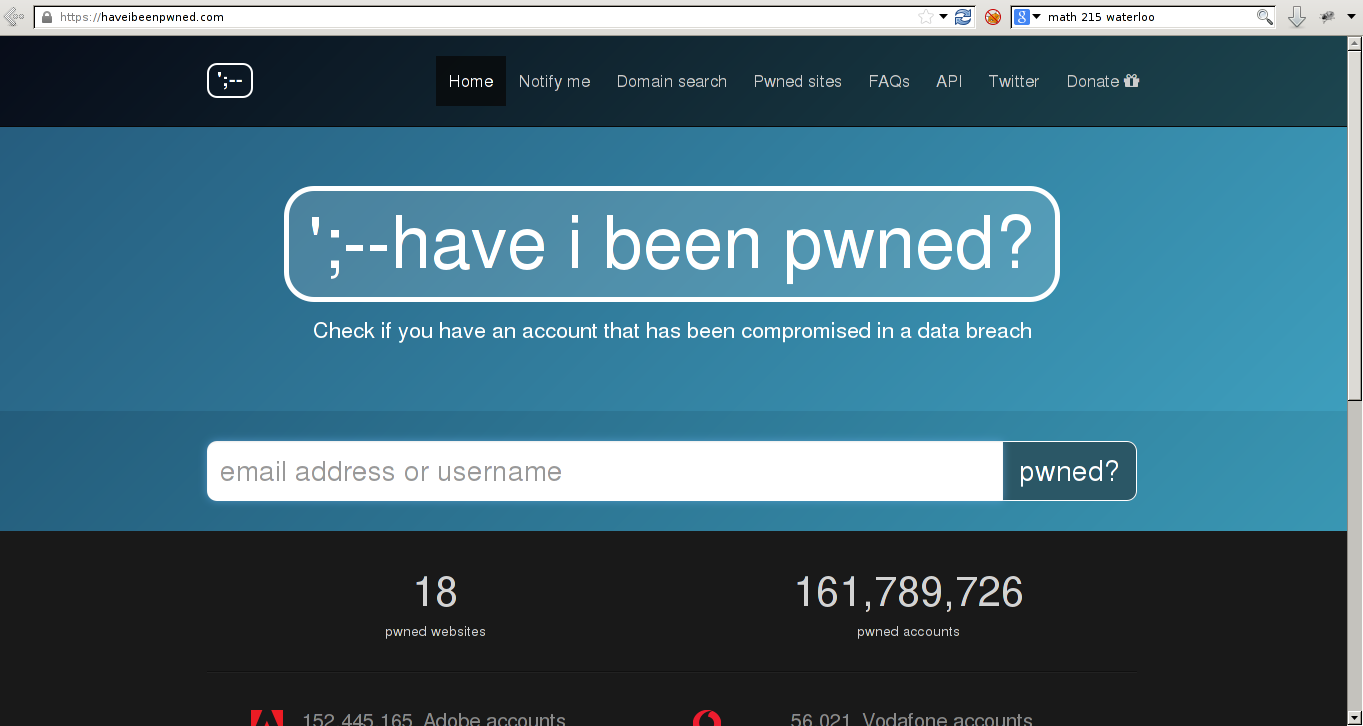
\includegraphics[width=0.75\textwidth]{images/haveibeenpwned.png}
\end{center}


\end{frame}


\begin{frame}
\frametitle{All Too Easy}

The first thing is to try really common passwords.

You just might get a hit!

\begin{center}
	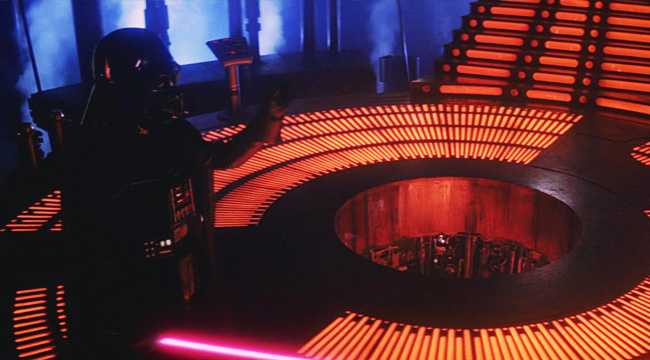
\includegraphics[width=0.7\textwidth]{images/alltooeasy.jpg}
\end{center}

``All too easy.''

\end{frame}


%%%%%%%%%%%%%%%%%%%%%%%%%%%%%%%%%%%%%%%%%%%%%%%%%%%%%%%%%%%%%%%%%%%%%%%%%%%%%%%%
\begin{frame}
  \frametitle{Breaking the Hash}
  
    How can we reverse the hash function?
    \begin{itemize}
    \item    Brute force.
    \end{itemize}~\\
    GPUs (or custom hardware) are good at that!
  
\end{frame}
%%%%%%%%%%%%%%%%%%%%%%%%%%%%%%%%%%%%%%%%%%%%%%%%%%%%%%%%%%%%%%%%%%%%%%%%%%%%%%%%

%%%%%%%%%%%%%%%%%%%%%%%%%%%%%%%%%%%%%%%%%%%%%%%%%%%%%%%%%%%%%%%%%%%%%%%%%%%%%%%%
\begin{frame}
  \frametitle{The Arms Race: Making Cracking Difficult}
  
    Historically: force repeated iterations of hashing.\\[1em]

    Main idea behind scrypt (hence DogeCoin):
    \begin{itemize}
    \item make hashing expensive in time and space.
    \end{itemize}~\\
    Implication: require more circuitry to break passwords.\\
    Increases both \# of operations and cost of brute-forcing.
  
\end{frame}
%%%%%%%%%%%%%%%%%%%%%%%%%%%%%%%%%%%%%%%%%%%%%%%%%%%%%%%%%%%%%%%%%%%%%%%%%%%%%%%%



\begin{frame}
\frametitle{Obligatory xkcd}

Of course, there's always this form of cracking:
\begin{center}
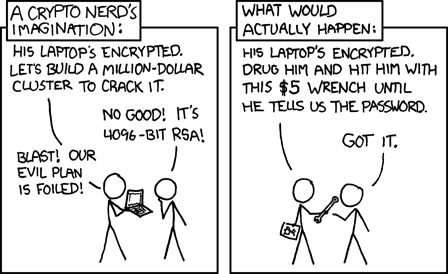
\includegraphics[width=0.75\textwidth]{images/xkcd-538}\\
\hfill (Source: xkcd 538)
\end{center}

\end{frame}


%%%%%%%%%%%%%%%%%%%%%%%%%%%%%%%%%%%%%%%%%%%%%%%%%%%%%%%%%%%%%%%%%%%%%%%%%%%%%%%%
\begin{frame}
  \frametitle{Formalizing ``expensive in time and space''}
  
    Want to force use of the ``most memory possible'' for a given
    number of operations.\\[1em]
  
    \begin{defn}
      A \emph{memory-hard} algorithm on a Random Access Machine is an
      algorithm which uses $S(n)$ space and $T(n)$ operations, where
      $S(n) \in \Omega(T(n)^{1-\varepsilon})$.
    \end{defn}~\\
    
      Such algorithms are expensive to implement in either hardware or software.
    

\end{frame}
%%%%%%%%%%%%%%%%%%%%%%%%%%%%%%%%%%%%%%%%%%%%%%%%%%%%%%%%%%%%%%%%%%%%%%%%%%%%%%%%

%%%%%%%%%%%%%%%%%%%%%%%%%%%%%%%%%%%%%%%%%%%%%%%%%%%%%%%%%%%%%%%%%%%%%%%%%%%%%%%%
\begin{frame}
  \frametitle{Generalizing to functions}
  
    Next, add a quantifier: \\move from particular algorithms to underlying functions.\\[1em]
    A \emph{sequential memory-hard function} is one where:

    \begin{itemize}
      \item the fastest
        sequential algorithm is memory-hard; and
      \item it is impossible for a
        parallel algorithm to asymptotically achieve lower cost.
    \end{itemize}
  
\end{frame}
%%%%%%%%%%%%%%%%%%%%%%%%%%%%%%%%%%%%%%%%%%%%%%%%%%%%%%%%%%%%%%%%%%%%%%%%%%%%%%%%

%%%%%%%%%%%%%%%%%%%%%%%%%%%%%%%%%%%%%%%%%%%%%%%%%%%%%%%%%%%%%%%%%%%%%%%%%%%%%%%%
\begin{frame}
  \frametitle{Not made of unicorn tears}
  
    \emph{Exhibit.} ReMix is a concrete example of a sequential memory hard function.\\[1em]
    The paper concludes with an example of a more realistic (cache-aware) model and
    a function in that context, BlockMix.
  
\end{frame}
%%%%%%%%%%%%%%%%%%%%%%%%%%%%%%%%%%%%%%%%%%%%%%%%%%%%%%%%%%%%%%%%%%%%%%%%%%%%%%%%


\begin{frame}
\frametitle{Across the Rainbow Bridge}

If designed well, hash functions aren't easy to brute force.

What if we remembered some previous work? 

It isn't practical, or possible, to store the hashes for every possible plaintext.

\end{frame}


\begin{frame}
\frametitle{Rainbow Table}

The rainbow table is a compromise between speed and space. 

The ``reduction'' function maps hashes to plaintext:

\begin{center}
	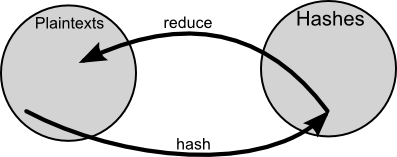
\includegraphics[width=0.7\textwidth]{images/rainbow-tables-reduce.png}
\end{center}

Example: \texttt{123456} $\rightarrow$ \texttt{d41d8cd98f00b204e9800998ecf8427e} $\rightarrow$ 418980

\end{frame}


\begin{frame}
\frametitle{Chain Formation}

\begin{center}
	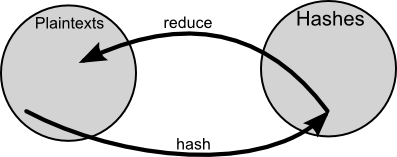
\includegraphics[width=0.7\textwidth]{images/rainbow-tables-reduce.png}
\end{center}

We should do this to develop some number of chains. 

This is the sort of task you could do with a GPU, because they can do a reduction relatively efficiently. 

\end{frame}


\begin{frame}
\frametitle{Or, y'know, just download them}

Once we have those developed for a specific input set and hash function, they can be re-used forever. 

You do not even need to make them yourself anymore (if you don't want) because you can download them on the internet... they are not hard to find. 

They are large, yes, but in the 25 - 900 GB range. 


\end{frame}


\begin{frame}
\frametitle{Rated 'S' for Suck}

\begin{center}
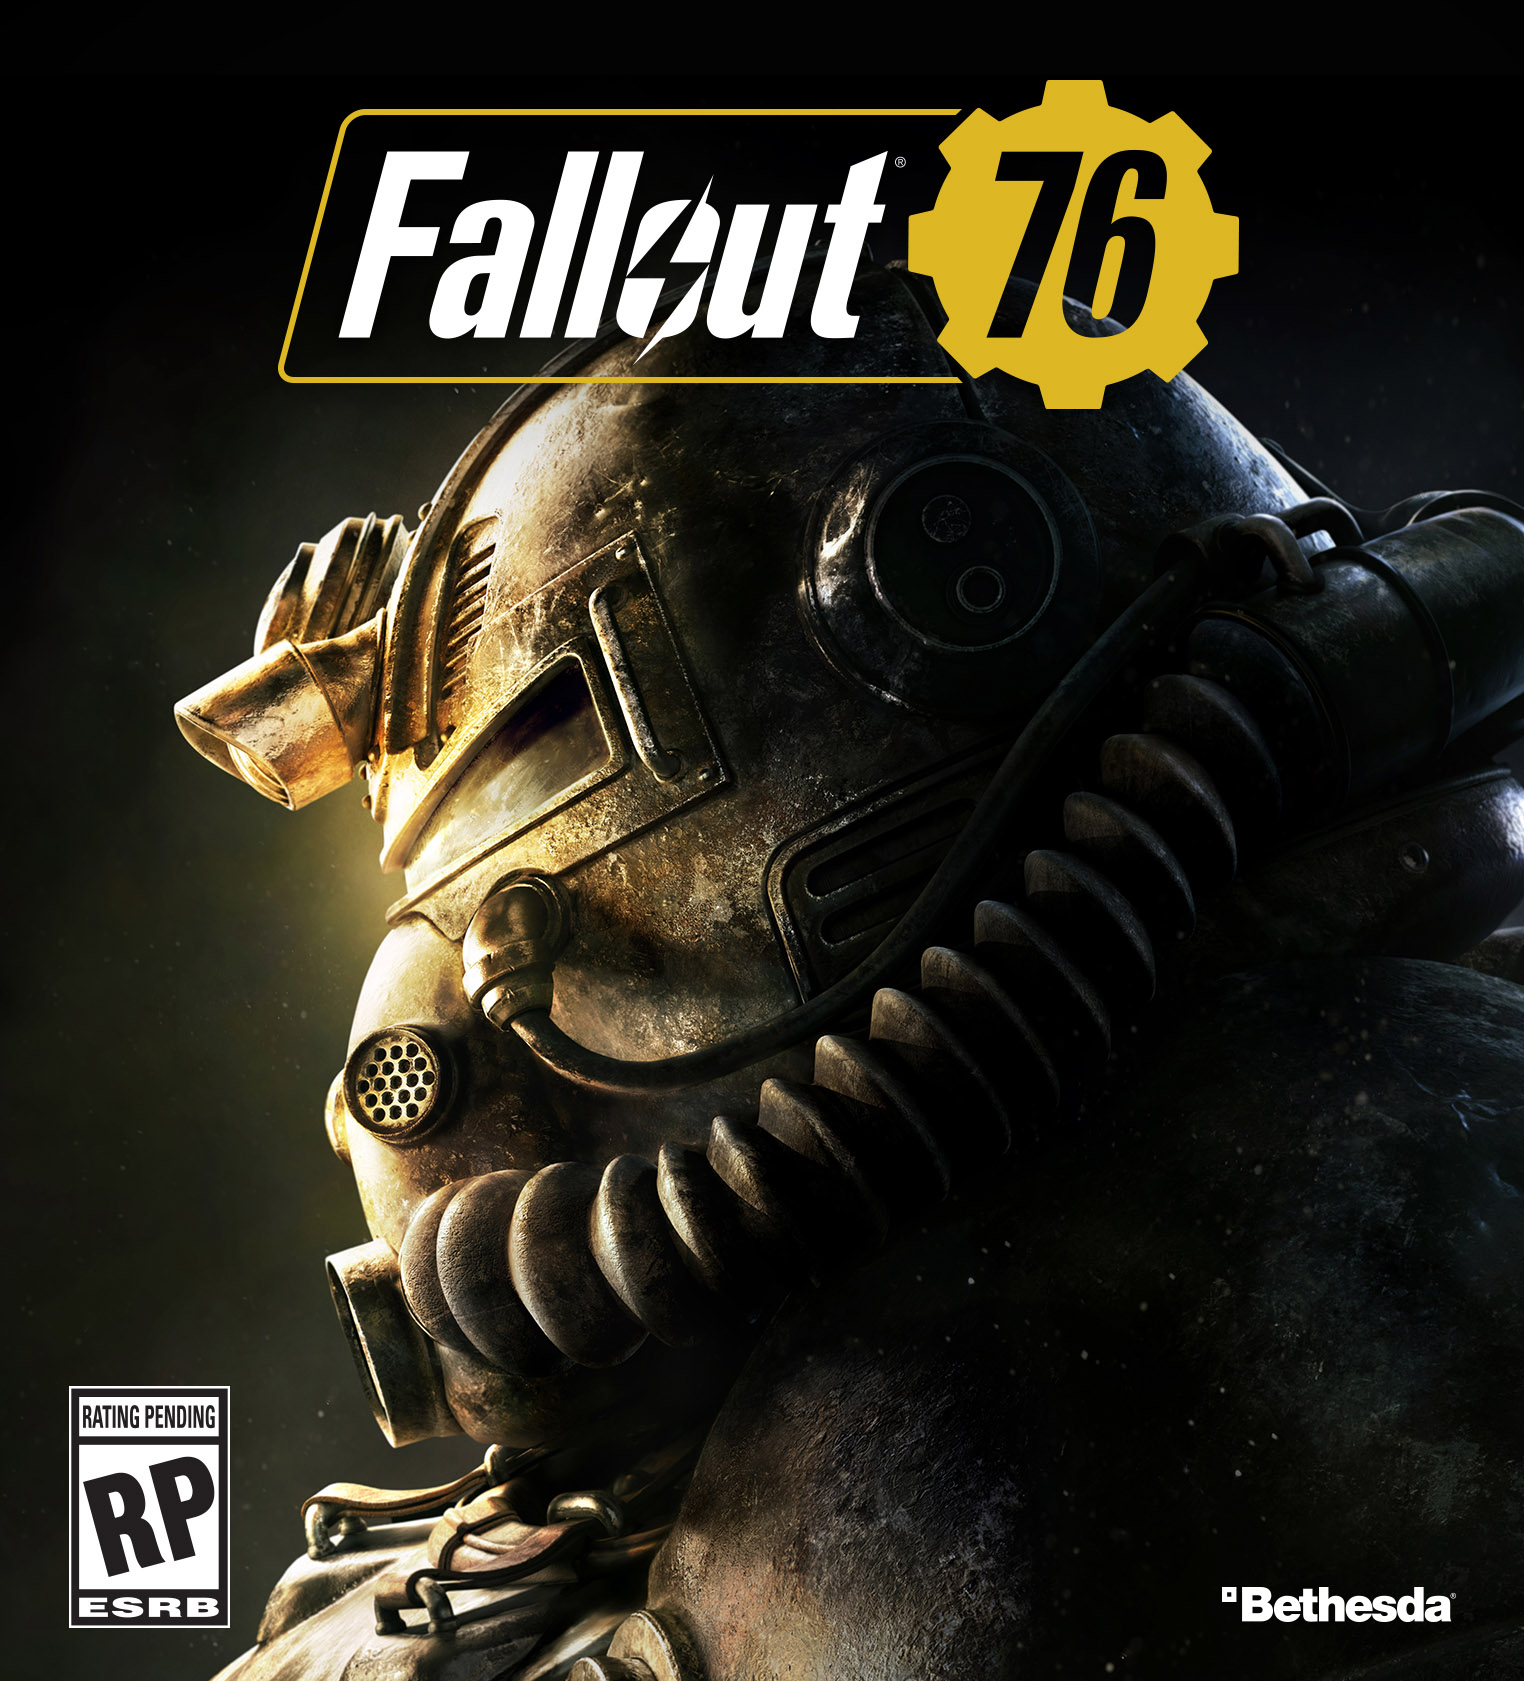
\includegraphics[width=0.3\textwidth]{images/Fallout_76_box_cover.jpg}
\end{center}

I mean, Fallout 76 had a day one patch of 52 GB, and it was a disaster of a game.

\end{frame}


\begin{frame}
\frametitle{How to Use Rainbow Tables}

\begin{enumerate}
	\item Look for the hash in the list of final hashes; if there, we are done
	\item If it's not there, reduce the hash into another plaintext and hash the new plaintext
	\item Go back to step 1
	\item If the hash matches a final hash, the chain with the match contains the original hash
	\item Having identified the correct chain, we can start at the beginning of the chain with the starting plaintext and hash, check to see if we are successful (if so, we are done); if not, reduce and try the next plaintext. 
\end{enumerate} 

\end{frame}


\begin{frame}
\frametitle{Is it Fast?}

Like generation, checking the tables can also be done efficiently by the GPU.

Some numbers from \url{http://www.cryptohaze.com/gpurainbowcracker.php.html}: 

\begin{itemize}
	\item Table generation on a GTX295 core for MD5 proceeds at around 430M links/sec.
	\item Cracking a password 'K\#n\&r4Z': real: 1m51.962s, user: 1m4.740s. sys: 0m15.320s
\end{itemize}

Yikes.

\end{frame}



\begin{frame}
\frametitle{The N-Body Simulation}

A common physics problem that programmers are asked to simulate is the N-Body problem.

\begin{center}
\includegraphics[width=0.8\textwidth]{images/Galaxy_Cluster_sim.png}
\end{center}
\hfill Image Credit: Michael L. Umbricht 


\end{frame}


\begin{frame}
\frametitle{The N-Body Simulation}

Let's assume it's OpenCL converted and is optimized.

Can we use \texttt{float} instead of \texttt{double}?

What if we want more?

\end{frame}


\begin{frame}
\frametitle{Estimation is Okay}

Points that are far away contribute only very small forces. 

So you can estimate them (crudely). 

The idea is to divide the points into a number of ``bins'' which are cubes representing a locale of some sort. 

Then, compute the centre of mass for each bin. 

When calculating the forces: centre of mass for faraway bins; individual particles for nearby particles.


\end{frame}


\begin{frame}
\frametitle{This used to be an assignment... }

A more concrete explanation with an example: suppose the space  is divided into $[0, 1000]^3$, so we can take bins which are cubes of length 100. 

This gives 1000 bins. 

To increase the accuracy, what should we do?

To increase the speed, what should we do?

\end{frame}


\begin{frame}[fragile]
\frametitle{Compute Centre of Mass}

Compute all of the masses in parallel: create one thread per bin, and add a point's
position if it belongs to the bin:

\begin{lstlisting}
    int xbin, ybin, zbin; // initialize with bin coordinates
    int b;
    for (i = 0; i < POINTS; i++) {
        if (pts[i] in bin coordinates) {
            cm[b].x += pts[i].x; // y, z too
            cm[b].w += 1.0f;
        }
    }
    cm[b].x /= cm[b].w; // etc
\end{lstlisting}

Note that this parallelizes with the number of bins.


\end{frame}


\begin{frame}
\frametitle{Map Points}

For the next step, the program needs to keep track of the points in
each bin. 

 In a second phase,
iterate over all bins again, this time putting coordinates into the
proper element of {\tt binPts}.

\end{frame}

\begin{frame}
\frametitle{Save Time}

The payoff from all these calculations is to save time while calculating forces. 

In this example, we'll compute exact forces for the points in the same bin and the directly-adjacent bins in each direction

That makes 27 bins in all, with 6 bins sharing a square, 12 bins sharing an edge, and 8 bins sharing a point with the centre bin). 

If there is no adjacent bin 
(i.e., this is an edge), just act as if there are no points 
in the place where the nonexistent bin would be. 

\end{frame}


\begin{frame}
\frametitle{More Overhead}

Necessarily, writing the program like this is going to mean more than one kernel.

This does mean there is overhead for each kernel, meaning the total amount of overhead goes up. 

Is it worth it? 

With 500*64 points:
\begin{itemize}
\item    OpenCL, no approximations (1 kernel): 0.182s
\item    OpenCL, with approximations (3 kernels): 0.168s
\end{itemize}

With 5000*64 points:
\begin{itemize}
\item    OpenCL, no approximations (1 kernel): 6.131s
\item    OpenCL, with approximations (3 kernels): 3.506s
\end{itemize}


\end{frame}




%%%%%%%%%%%%%%%%%%%%%%%%%%%%%%%%%%%%%%%%%%%%%%%%%%%%%%%%%%%%%%%%%%%%%%%%%%%%%%%%
\begin{frame}
  \frametitle{Trading Accuracy for Performance}


    Consider Monte Carlo integration.\\
    It illustrates a general tradeoff: accuracy vs performance.\\
  
    Martin Rinard generalized the accuracy vs performance tradeoff with:
      \begin{itemize}
        \item early phase termination [OOPSLA07]
        \item loop perforation [CSAIL TR 2009]
      \end{itemize}

\end{frame}
%%%%%%%%%%%%%%%%%%%%%%%%%%%%%%%%%%%%%%%%%%%%%%%%%%%%%%%%%%%%%%%%%%%%%%%%%%%%%%%%


%%%%%%%%%%%%%%%%%%%%%%%%%%%%%%%%%%%%%%%%%%%%%%%%%%%%%%%%%%%%%%%%%%%%%%%%%%%%%%%%
\begin{frame}
  \frametitle{Early Phase Termination}



  We've seen barriers before.\\

  No thread may proceed past a barrier until all of the threads
reach the barrier.\\[1em]

  This may slow down the program: maybe one of the threads is horribly
  slow.\\[1em]

  Solution: kill the slowest thread.


\end{frame}
%%%%%%%%%%%%%%%%%%%%%%%%%%%%%%%%%%%%%%%%%%%%%%%%%%%%%%%%%%%%%%%%%%%%%%%%%%%%%%%%

%%%%%%%%%%%%%%%%%%%%%%%%%%%%%%%%%%%%%%%%%%%%%%%%%%%%%%%%%%%%%%%%%%%%%%%%%%%%%%%%
\begin{frame}
  \frametitle{Early Phase Termination: Objection}

\Huge
\begin{center}
``Oh no, that's going to change the meaning of the program!''
\end{center}
\end{frame}
%%%%%%%%%%%%%%%%%%%%%%%%%%%%%%%%%%%%%%%%%%%%%%%%%%%%%%%%%%%%%%%%%%%%%%%%%%%%%%%%

%%%%%%%%%%%%%%%%%%%%%%%%%%%%%%%%%%%%%%%%%%%%%%%%%%%%%%%%%%%%%%%%%%%%%%%%%%%%%%%%
\begin{frame}
  \frametitle{Early Phase Termination: When is it OK anyway?}


OK, so we don't want to be completely crazy.\\[1em]

Instead: 
\begin{itemize}
\item develop a statistical model of the program behaviour.
\item only kill tasks that don't introduce unacceptable distortions.
\end{itemize}

~\\[1em]

When we run the program: \\ \qquad get the output, plus a confidence interval.



\end{frame}
%%%%%%%%%%%%%%%%%%%%%%%%%%%%%%%%%%%%%%%%%%%%%%%%%%%%%%%%%%%%%%%%%%%%%%%%%%%%%%%%

%%%%%%%%%%%%%%%%%%%%%%%%%%%%%%%%%%%%%%%%%%%%%%%%%%%%%%%%%%%%%%%%%%%%%%%%%%%%%%%%
\begin{frame}
  \frametitle{Early Phase Termination: Two Examples}



Monte Carlo simulators: \\
Raytracers:
\begin{itemize}
\item already picking points randomly.
\end{itemize}

In both cases: spawn a lot of threads.\\[1em]
Could wait for all threads to complete;\\
or just compensate for missing data points,\\
assuming they look like points you did compute.


\end{frame}
%%%%%%%%%%%%%%%%%%%%%%%%%%%%%%%%%%%%%%%%%%%%%%%%%%%%%%%%%%%%%%%%%%%%%%%%%%%%%%%%

%%%%%%%%%%%%%%%%%%%%%%%%%%%%%%%%%%%%%%%%%%%%%%%%%%%%%%%%%%%%%%%%%%%%%%%%%%%%%%%%
\begin{frame}
  \frametitle{Early Phase Termination: Another Justification}



In scientific computations:
\begin{itemize}
\item using points that were measured (subject to error);
\item computing using machine numbers (also with error). 
\end{itemize}

Computers are only providing simulations, not ground truth.

Actual question: is the simulation is good enough?

\end{frame}

%%%%%%%%%%%%%%%%%%%%%%%%%%%%%%%%%%%%%%%%%%%%%%%%%%%%%%%%%%%%%%%%%%%%%%%%%%%%%%%%

%%%%%%%%%%%%%%%%%%%%%%%%%%%%%%%%%%%%%%%%%%%%%%%%%%%%%%%%%%%%%%%%%%%%%%%%%%%%%%%%
\begin{frame}[fragile]
  \frametitle{Loop Perforation}


  Like early-phase termination, but for sequential programs:\\
  \qquad throw away data that's not actually useful.

  \begin{lstlisting}
for (i = 0; i < n; ++i) sum += numbers[i];
  \end{lstlisting}

  \begin{center}
    $\Downarrow$
  \end{center}

  \begin{lstlisting}
for (i = 0; i < n; i += 2) sum += numbers[i];
sum *= 2;
  \end{lstlisting}

  This gives a speedup of $\sim$ 2 if {\tt numbers[]} is nice.\\[1em]

  Works for video encoding: can't observe difference.



\end{frame}
%%%%%%%%%%%%%%%%%%%%%%%%%%%%%%%%%%%%%%%%%%%%%%%%%%%%%%%%%%%%%%%%%%%%%%%%%%%%%%%%

%%%%%%%%%%%%%%%%%%%%%%%%%%%%%%%%%%%%%%%%%%%%%%%%%%%%%%%%%%%%%%%%%%%%%%%%%%%%%%%%
\begin{frame}
  \frametitle{Applications of Reduced Resource Computation}


  Loop perforation works for:
  \begin{itemize}
   \item evaluating forces on water molecules (summing numbers);
   \item Monte-Carlo simulation of swaption pricing;
   \item video encoding.
  \end{itemize}

  More on the video encoding example:\\
  Changing loop increments from 4 to 8 gives:
\begin{itemize}
 \item speedup of 1.67;
 \item signal-to-noise ratio decrease of 0.87\%;
 \item bitrate increase of 18.47\%;
 \item visually indistinguishable results.
\end{itemize}

\end{frame}

%%%%%%%%%%%%%%%%%%%%%%%%%%%%%%%%%%%%%%%%%%%%%%%%%%%%%%%%%%%%%%%%%%%%%%%%%%%%%%%%

%%%%%%%%%%%%%%%%%%%%%%%%%%%%%%%%%%%%%%%%%%%%%%%%%%%%%%%%%%%%%%%%%%%%%%%%%%%%%%%%
\begin{frame}[fragile]
  \frametitle{Video Encoding Skeleton Code}


\begin{lstlisting}
min = DBL_MAX;
index = 0;
for (i = 0; i < m; i++) {
  sum = 0;
  for (j = 0; j < n; j++) sum += numbers[i][j];
  if (min < sum) {
    min = sum;
    index = i;
  }
}
\end{lstlisting}
The optimization changes the loop increments and then compensates. 

\end{frame}

%%%%%%%%%%%%%%%%%%%%%%%%%%%%%%%%%%%%%%%%%%%%%%%%%%%%%%%%%%%%%%%%%%%%%%%%%%%%%%%%


\end{document}

